\documentclass[aspectratio=43]{beamer}

% Text packages to stop warnings
\usepackage{lmodern}
\usepackage{textcomp}
\usepackage{ulem}
\usepackage[utf8]{inputenc}
\usepackage[T1]{fontenc}

\usepackage{listings}
\usepackage{tikz}
\usetikzlibrary{arrows,decorations.pathreplacing,positioning}

% Themes
\usetheme{Boadilla}
\setbeamertemplate{footline}[page number]{}
\setbeamertemplate{navigation symbols}{}

% Suppress the navigation bar
\beamertemplatenavigationsymbolsempty

\newenvironment{changemargin}[1]{% 
  \begin{list}{}{% 
    \setlength{\topsep}{0pt}% 
    \setlength{\leftmargin}{#1}% 
    \setlength{\rightmargin}{1em}
    \setlength{\listparindent}{\parindent}% 
    \setlength{\itemindent}{\parindent}% 
    \setlength{\parsep}{\parskip}% 
  }% 
  \item[]}{\end{list}} 

\lstset{basicstyle=\scriptsize, frame=single}

\lstdefinelanguage{JavaScript}{
  keywords={typeof, new, true, false, catch, function, return, null, catch, switch, var, if, in, while, do, else, case, break},
  keywordstyle=\color{blue}\bfseries,
  ndkeywords={class, export, boolean, throw, implements, import, this},
  ndkeywordstyle=\color{darkgray}\bfseries,
  identifierstyle=\color{black},
  sensitive=false,
  comment=[l]{//},
  morecomment=[s]{/*}{*/},
  commentstyle=\color{purple}\ttfamily,
  stringstyle=\color{red}\ttfamily,
  morestring=[b]',
  morestring=[b]"
}

\title{Lecture 26---More Profiling: gperftools, \\ systemwide tools: oprofile, perf, DTrace, etc.}
\subtitle{ECE 459: Programming for Performance}
\date{March 11, 2015}

\begin{document}
%%%%%%%%%%%%%%%%%%%%%%%%%%%%%%%%%%%%%%%%%%%%%%%%%%%%%%%%%%%%%%%%%%%%%%%%%%%%%%%%
\begin{frame}[plain]
  \titlepage
\end{frame}
%%%%%%%%%%%%%%%%%%%%%%%%%%%%%%%%%%%%%%%%%%%%%%%%%%%%%%%%%%%%%%%%%%%%%%%%%%%%%%%%

\part{gperftools}
\frame{\partpage}

%%%%%%%%%%%%%%%%%%%%%%%%%%%%%%%%%%%%%%%%%%%%%%%%%%%%%%%%%%%%%%%%%%%%%%%%%%%%%%%%
\begin{frame}
  \frametitle{Introduction to gperftools}

  \begin{changemargin}{2cm}
    Google Performance Tools include:
      
      \begin{itemize}
        \item CPU profiler.
        \item Heap profiler.
        \item Heap checker.
        \item Faster (multithreaded) {\tt malloc}.
      \end{itemize}
~\\[1em]
     We'll mostly use the CPU profiler:
      \begin{itemize}
        \item purely statistical sampling;
        \item no recompilation; at most linking; and
        \item built-in visual output.
      \end{itemize}
  \end{changemargin}
\end{frame}
%%%%%%%%%%%%%%%%%%%%%%%%%%%%%%%%%%%%%%%%%%%%%%%%%%%%%%%%%%%%%%%%%%%%%%%%%%%%%%%%

%%%%%%%%%%%%%%%%%%%%%%%%%%%%%%%%%%%%%%%%%%%%%%%%%%%%%%%%%%%%%%%%%%%%%%%%%%%%%%%%
\begin{frame}[fragile]
  \frametitle{Google Perf Tools profiler usage}

  \begin{changemargin}{2cm}
    You can use the profiler without any recompilation.
      \begin{itemize}
        \item Not recommended---worse data.
      \end{itemize}

  \begin{lstlisting}
LD_PRELOAD="/usr/lib/libprofiler.so" \
CPUPROFILE=test.prof ./test
  \end{lstlisting}

     The other option is to link to the profiler:
      \begin{itemize}
        \item {\tt -lprofiler}
      \end{itemize}
    Both options read the {\tt CPUPROFILE} environment variable:
      \begin{itemize}
        \item states the location to write the profile data.
      \end{itemize}
  \end{changemargin}
\end{frame}
%%%%%%%%%%%%%%%%%%%%%%%%%%%%%%%%%%%%%%%%%%%%%%%%%%%%%%%%%%%%%%%%%%%%%%%%%%%%%%%%

%%%%%%%%%%%%%%%%%%%%%%%%%%%%%%%%%%%%%%%%%%%%%%%%%%%%%%%%%%%%%%%%%%%%%%%%%%%%%%%%
\begin{frame}[fragile]
  \frametitle{Other Usage}

  \begin{changemargin}{2cm}
     You can use the profiling library directly as well:
      \begin{itemize}
        \item {\tt \#include <gperftools/profiler.h>}
      \end{itemize}
     Bracket code you want profiled with:
      \begin{itemize}
        \item {\tt ProfilerStart()}
        \item {\tt ProfilerEnd()}
      \end{itemize}~\\
    
    You can change the sampling frequency with the
      {\tt CPUPROFILE\_FREQUENCY} environment variable.
      \begin{itemize}
        \item {\bf Default value:} 100
      \end{itemize}
  \end{changemargin}
\end{frame}
%%%%%%%%%%%%%%%%%%%%%%%%%%%%%%%%%%%%%%%%%%%%%%%%%%%%%%%%%%%%%%%%%%%%%%%%%%%%%%%%

%%%%%%%%%%%%%%%%%%%%%%%%%%%%%%%%%%%%%%%%%%%%%%%%%%%%%%%%%%%%%%%%%%%%%%%%%%%%%%%%
\begin{frame}[fragile]
  \frametitle{{\tt pprof} Usage}

  \begin{changemargin}{1.5cm}
    Like {\tt gprof}, it will analyze profiling results.

  \begin{lstlisting}
% pprof test test.prof
    Enters "interactive" mode
% pprof --text test test.prof
    Outputs one line per procedure
% pprof --gv test test.prof
     Displays annotated call-graph via 'gv'
% pprof --gv --focus=Mutex test test.prof
    Restricts to code paths including a .*Mutex.* entry
% pprof --gv --focus=Mutex --ignore=string test test.prof
    Code paths including Mutex but not string
% pprof --list=getdir test test.prof
    (Per-line) annotated source listing for getdir()
% pprof --disasm=getdir test test.prof
    (Per-PC) annotated disassembly for getdir()
  \end{lstlisting}

    Can also output {\tt dot}, {\tt ps}, {\tt pdf} or {\tt gif} instead of
      {\tt gv}.
  \end{changemargin}

\end{frame}
%%%%%%%%%%%%%%%%%%%%%%%%%%%%%%%%%%%%%%%%%%%%%%%%%%%%%%%%%%%%%%%%%%%%%%%%%%%%%%%%

%%%%%%%%%%%%%%%%%%%%%%%%%%%%%%%%%%%%%%%%%%%%%%%%%%%%%%%%%%%%%%%%%%%%%%%%%%%%%%%%
\begin{frame}[fragile]
  \frametitle{Text Output}

  \begin{changemargin}{1.5cm}
    Similar to the flat profile in {\tt gprof}

  \begin{lstlisting}
jon@riker examples master % pprof --text test test.prof 
Using local file test.
Using local file test.prof.
Removing killpg from all stack traces.
Total: 300 samples
      95  31.7%  31.7%      102  34.0% int_power
      58  19.3%  51.0%       58  19.3% float_power
      51  17.0%  68.0%       96  32.0% float_math_helper
      50  16.7%  84.7%      137  45.7% int_math_helper
      18   6.0%  90.7%      131  43.7% float_math
      14   4.7%  95.3%      159  53.0% int_math
      14   4.7% 100.0%      300 100.0% main
       0   0.0% 100.0%      300 100.0% __libc_start_main
       0   0.0% 100.0%      300 100.0% _start
  \end{lstlisting}
  \end{changemargin}

\end{frame}
%%%%%%%%%%%%%%%%%%%%%%%%%%%%%%%%%%%%%%%%%%%%%%%%%%%%%%%%%%%%%%%%%%%%%%%%%%%%%%%%

%%%%%%%%%%%%%%%%%%%%%%%%%%%%%%%%%%%%%%%%%%%%%%%%%%%%%%%%%%%%%%%%%%%%%%%%%%%%%%%%
\begin{frame}
  \frametitle{Text Output Explained}

  \begin{changemargin}{2cm}
    Columns, from left to right:\\[1em]

    Number of checks (samples) in this function.\\
    Percentage of checks in this function.
      \begin{itemize}
        \item Same as {\bf time} in {\tt gprof}.\\[1em]
      \end{itemize}
    Percentage of checks in the functions printed so far.
      \begin{itemize}
        \item Equivalent to {\bf cumulative} (but in \%).\\[1em]
      \end{itemize}
    Number of checks in this function and its callees.\\
    Percentage of checks in this function and its callees.\\
    Function name.
  \end{changemargin}
\end{frame}
%%%%%%%%%%%%%%%%%%%%%%%%%%%%%%%%%%%%%%%%%%%%%%%%%%%%%%%%%%%%%%%%%%%%%%%%%%%%%%%%

%%%%%%%%%%%%%%%%%%%%%%%%%%%%%%%%%%%%%%%%%%%%%%%%%%%%%%%%%%%%%%%%%%%%%%%%%%%%%%%%
\begin{frame}
  \frametitle{Graphical Output}

  \begin{center}
    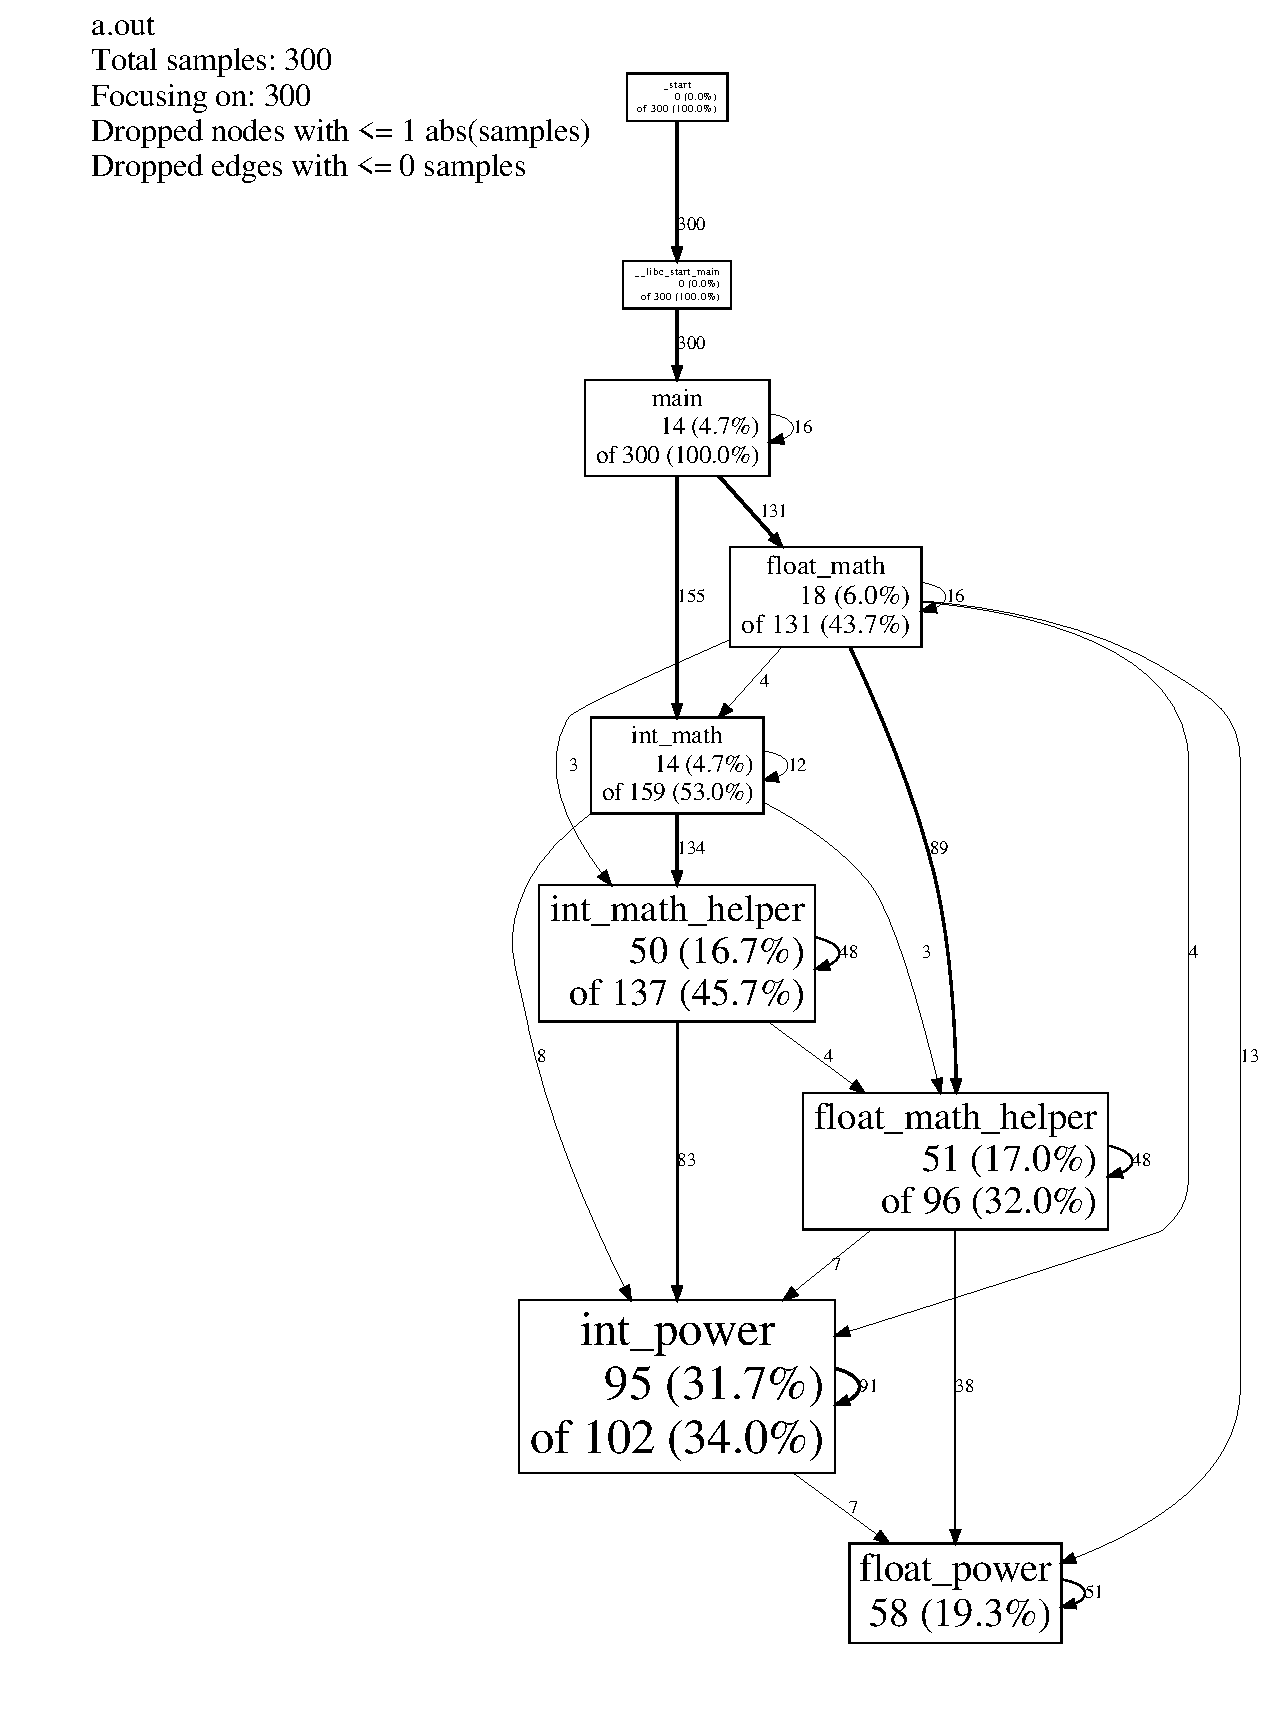
\includegraphics[scale=0.25]{L26/test}
  \end{center}
\end{frame}
%%%%%%%%%%%%%%%%%%%%%%%%%%%%%%%%%%%%%%%%%%%%%%%%%%%%%%%%%%%%%%%%%%%%%%%%%%%%%%%%

%%%%%%%%%%%%%%%%%%%%%%%%%%%%%%%%%%%%%%%%%%%%%%%%%%%%%%%%%%%%%%%%%%%%%%%%%%%%%%%%
\begin{frame}
  \frametitle{Graphical Output Explained}

  \begin{changemargin}{2cm}
  Output was too small to read on the slide.

  \begin{itemize}
    \item Shows the same numbers as the text output.
    \item Directed edges denote function calls.
    \item Note: number of samples in callees = \\
      \qquad number in ``this function + callees'' - \\
      \qquad number in ``this function''.\\
    \item {\bf Example:}\\
{{\tt float\_math\_helper}, 51 (local) of 96 (cumulative)} \\
      96 - 51 = 45 (callees)
      \begin{itemize}
        \item callee {\tt int\_power} = 7 (bogus)
        \item callee {\tt float\_power} = 38
        \item callees total = 45
      \end{itemize}

  \end{itemize}
  \end{changemargin}
\end{frame}
%%%%%%%%%%%%%%%%%%%%%%%%%%%%%%%%%%%%%%%%%%%%%%%%%%%%%%%%%%%%%%%%%%%%%%%%%%%%%%%%

%%%%%%%%%%%%%%%%%%%%%%%%%%%%%%%%%%%%%%%%%%%%%%%%%%%%%%%%%%%%%%%%%%%%%%%%%%%%%%%%
\begin{frame}
  \frametitle{Things You May Notice}

  \begin{changemargin}{2cm}
    Call graph is not exact.
    
      \begin{itemize}
        \item In fact, it shows many bogus relations which clearly don't exist.
        \item For instance, we know that there are no cross-calls between {\tt int} and {\tt float} functions.
      \end{itemize}~\\

    As with {\tt gprof}, optimizations will change the
      graph.\\[1em]

    You'll probably want to look at the text profile first, then use the
      {\tt --focus} flag to look at individual functions.
  \end{changemargin}
\end{frame}
%%%%%%%%%%%%%%%%%%%%%%%%%%%%%%%%%%%%%%%%%%%%%%%%%%%%%%%%%%%%%%%%%%%%%%%%%%%%%%%%

% How to Read
% http://www.cs.utah.edu/dept/old/texinfo/as/gprof.html
% http://www.civilnet.cn/book/kernel/GNU.Linux.Application.Programming/LiB0055.html
% http://ececmpsysweb.groups.et.byu.net/cmpsys.2004.winter/citizenship/Bryan_Wheeler/Profiling_Tutorial.html

% gprof
% OProfile
% Valgrind
% Intel VTune
% AMD CodeAnalyst

\part{System profiling: oprofile,~perf,~DTrace,~WAIT}
\frame{\partpage}

%%%%%%%%%%%%%%%%%%%%%%%%%%%%%%%%%%%%%%%%%%%%%%%%%%%%%%%%%%%%%%%%%%%%%%%%%%%%%%%%
\begin{frame}
  \frametitle{Introduction: oprofile}

\begin{changemargin}{2cm}
    \url{http://oprofile.sourceforge.net}\\[1em]

    Sampling-based tool.\\[1em]
    
    Uses CPU performance counters.\\[1em]

    Tracks currently-running function;\\
    records profiling data for every application run.\\[1em]

    Can work system-wide (across processes).\\[1em]

    Technology: Linux Kernel Performance Events\\ (formerly a Linux kernel module).
\end{changemargin}
\end{frame}
%%%%%%%%%%%%%%%%%%%%%%%%%%%%%%%%%%%%%%%%%%%%%%%%%%%%%%%%%%%%%%%%%%%%%%%%%%%%%%%%

%%%%%%%%%%%%%%%%%%%%%%%%%%%%%%%%%%%%%%%%%%%%%%%%%%%%%%%%%%%%%%%%%%%%%%%%%%%%%%%%
\begin{frame}[fragile]
  \frametitle{Setting up {\tt oprofile}}

\begin{changemargin}{2cm}
  Must run as root to use system-wide, otherwise can use per-process.

  \begin{lstlisting}
% sudo opcontrol \
     --vmlinux=/usr/src/linux-3.2.7-1-ARCH/vmlinux
% echo 0 | sudo tee /proc/sys/kernel/nmi_watchdog
% sudo opcontrol --start
Using default event: CPU_CLK_UNHALTED:100000:0:1:1
Using 2.6+ OProfile kernel interface.
Reading module info.
Using log file /var/lib/oprofile/samples/oprofiled.log
Daemon started.
Profiler running.
  \end{lstlisting}

  Per-process:
\begin{lstlisting}
[plam@lynch nm-morph]$ operf ./test_harness
operf: Profiler started

Profiling done.
\end{lstlisting}%$

\end{changemargin}
\end{frame}
%%%%%%%%%%%%%%%%%%%%%%%%%%%%%%%%%%%%%%%%%%%%%%%%%%%%%%%%%%%%%%%%%%%%%%%%%%%%%%%%

%%%%%%%%%%%%%%%%%%%%%%%%%%%%%%%%%%%%%%%%%%%%%%%%%%%%%%%%%%%%%%%%%%%%%%%%%%%%%%%%
\begin{frame}[fragile]
  \frametitle{{\tt oprofile} Usage (1)}
  
\begin{changemargin}{1cm}
  Pass your executable to {\tt opreport}.

  \begin{lstlisting}
% sudo opreport -l ./test    
CPU: Intel Core/i7, speed 1595.78 MHz (estimated)
Counted CPU_CLK_UNHALTED events (Clock cycles when not
halted) with a unit mask of 0x00 (No unit mask) count 100000
samples  %        symbol name
7550     26.0749  int_math_helper
5982     20.6596  int_power
5859     20.2348  float_power
3605     12.4504  float_math
3198     11.0447  int_math
2601      8.9829  float_math_helper
160       0.5526  main
  \end{lstlisting}
  
    If you have debug symbols ({\tt -g}) you could use:

  \begin{lstlisting}
% sudo opannotate --source \
--output-dir=/path/to/annotated-source /path/to/mybinary
  \end{lstlisting}
\end{changemargin}
\end{frame}
%%%%%%%%%%%%%%%%%%%%%%%%%%%%%%%%%%%%%%%%%%%%%%%%%%%%%%%%%%%%%%%%%%%%%%%%%%%%%%%%

%%%%%%%%%%%%%%%%%%%%%%%%%%%%%%%%%%%%%%%%%%%%%%%%%%%%%%%%%%%%%%%%%%%%%%%%%%%%%%%%
\begin{frame}[fragile]
  \frametitle{{\tt oprofile} Usage (2)}
  
\begin{changemargin}{2cm}
    Use {\tt opreport} by itself for a whole-system view.\\
    You can also reset and stop the profiling.

  \begin{lstlisting}
% sudo opcontrol --reset 
Signalling daemon... done
% sudo opcontrol --stop
Stopping profiling.
  \end{lstlisting}
\end{changemargin}
\end{frame}
%%%%%%%%%%%%%%%%%%%%%%%%%%%%%%%%%%%%%%%%%%%%%%%%%%%%%%%%%%%%%%%%%%%%%%%%%%%%%%%%

%%%%%%%%%%%%%%%%%%%%%%%%%%%%%%%%%%%%%%%%%%%%%%%%%%%%%%%%%%%%%%%%%%%%%%%%%%%%%%%%
\begin{frame}
  \frametitle{Perf: Introduction}

\begin{changemargin}{1cm}
    \url{https://perf.wiki.kernel.org/index.php/Tutorial}\\[1em]

    Interface to Linux kernel built-in sampling-based profiling.\\
    Per-process, per-CPU, or system-wide.\\
    Can even report the cost of each line of code.
\end{changemargin}
\end{frame}
%%%%%%%%%%%%%%%%%%%%%%%%%%%%%%%%%%%%%%%%%%%%%%%%%%%%%%%%%%%%%%%%%%%%%%%%%%%%%%%%

%%%%%%%%%%%%%%%%%%%%%%%%%%%%%%%%%%%%%%%%%%%%%%%%%%%%%%%%%%%%%%%%%%%%%%%%%%%%%%%%
\begin{frame}[fragile]
  \frametitle{Perf: Usage Example}

On last year's Assignment 3 code:
\begin{lstlisting}[basicstyle=\tiny]
[plam@lynch nm-morph]$ perf stat ./test_harness

 Performance counter stats for './test_harness':

       6562.501429 task-clock                #    0.997 CPUs utilized          
               666 context-switches          #    0.101 K/sec                  
                 0 cpu-migrations            #    0.000 K/sec                  
             3,791 page-faults               #    0.578 K/sec                  
    24,874,267,078 cycles                    #    3.790 GHz                     [83.32%]
    12,565,457,337 stalled-cycles-frontend   #   50.52% frontend cycles idle    [83.31%]
     5,874,853,028 stalled-cycles-backend    #   23.62% backend  cycles idle    [66.63%]
    33,787,408,650 instructions              #    1.36  insns per cycle        
                                             #    0.37  stalled cycles per insn [83.32%]
     5,271,501,213 branches                  #  803.276 M/sec                   [83.38%]
       155,568,356 branch-misses             #    2.95% of all branches         [83.36%]

       6.580225847 seconds time elapsed
\end{lstlisting} %$
\end{frame}
%%%%%%%%%%%%%%%%%%%%%%%%%%%%%%%%%%%%%%%%%%%%%%%%%%%%%%%%%%%%%%%%%%%%%%%%%%%%%%%%

%%%%%%%%%%%%%%%%%%%%%%%%%%%%%%%%%%%%%%%%%%%%%%%%%%%%%%%%%%%%%%%%%%%%%%%%%%%%%%%%
\begin{frame}[fragile]
  \frametitle{Perf: Source-level Analysis}

\begin{changemargin}{2cm}
perf can tell you which instructions are taking time, or which lines of code.\\[1em]

Compile with {\tt -ggdb} to enable source code viewing.

\begin{lstlisting}
% perf record ./test_harness
% perf annotate
\end{lstlisting}

{\tt perf annotate} is interactive. Play around with it.
\end{changemargin}

\end{frame}
%%%%%%%%%%%%%%%%%%%%%%%%%%%%%%%%%%%%%%%%%%%%%%%%%%%%%%%%%%%%%%%%%%%%%%%%%%%%%%%%

%%%%%%%%%%%%%%%%%%%%%%%%%%%%%%%%%%%%%%%%%%%%%%%%%%%%%%%%%%%%%%%%%%%%%%%%%%%%%%%%
\begin{frame}
  \frametitle{DTrace: Introduction}

\begin{changemargin}{1cm}
    \url{http://queue.acm.org/detail.cfm?id=1117401}\\[1em]

    Intrumentation-based tool.\\
    System-wide.\\
    Meant to be used on production systems. (Eh?)\\[1em]
     \only<2>{
     {\small (Typical instrumentation can have a slowdown of 100x (Valgrind).)}\\
     Design goals:\\
\begin{enumerate} 
\item No overhead when not in use;
\item Guarantee safety---must not crash\\ \qquad (strict limits on expressiveness of probes).
\end{enumerate}
     }
\end{changemargin}
\end{frame}
%%%%%%%%%%%%%%%%%%%%%%%%%%%%%%%%%%%%%%%%%%%%%%%%%%%%%%%%%%%%%%%%%%%%%%%%%%%%%%%%

%%%%%%%%%%%%%%%%%%%%%%%%%%%%%%%%%%%%%%%%%%%%%%%%%%%%%%%%%%%%%%%%%%%%%%%%%%%%%%%%
\begin{frame}
  \frametitle{DTrace: Operation}

\begin{changemargin}{2cm}
    How does DTrace achieve 0 overhead?\\
\begin{itemize}
    \item only when activated, dynamically rewrites code by placing a branch to
      instrumentation code.
\end{itemize}

    Uninstrumented: runs as if nothing changed.\\[1em]

    Most instrumentation: at function entry or exit points.\\
    You can also instrument kernel functions, locking, instrument-based
      on other events.\\[1em]

    Can express sampling as instrumentation-based events also.
\end{changemargin}
\end{frame}
%%%%%%%%%%%%%%%%%%%%%%%%%%%%%%%%%%%%%%%%%%%%%%%%%%%%%%%%%%%%%%%%%%%%%%%%%%%%%%%%

%%%%%%%%%%%%%%%%%%%%%%%%%%%%%%%%%%%%%%%%%%%%%%%%%%%%%%%%%%%%%%%%%%%%%%%%%%%%%%%%
\begin{frame}[fragile]
  \frametitle{DTrace Example}

\begin{changemargin}{1cm}
  You write this:

  \begin{lstlisting}
syscall::read:entry {
    self->t = timestamp;
}

syscall::read:return
/self->t/ {
    printf("%d/%d spent %d nsecs in read\n"
           pid, tid, timestamp - self->t);
}
  \end{lstlisting}

    {\tt t} is a thread-local variable.\\
    This code prints how long each call to {\tt read} takes, along with
      context.\\[1em]
    To ensure safety, DTrace limits what you write; e.g. no loops.
      \begin{itemize}
        \item (Hence, no infinite loops!)
      \end{itemize}
\end{changemargin}

\end{frame}
%%%%%%%%%%%%%%%%%%%%%%%%%%%%%%%%%%%%%%%%%%%%%%%%%%%%%%%%%%%%%%%%%%%%%%%%%%%%%%%%

%%%%%%%%%%%%%%%%%%%%%%%%%%%%%%%%%%%%%%%%%%%%%%%%%%%%%%%%%%%%%%%%%%%%%%%%%%%%%%%%
\begin{frame}[fragile]
  \frametitle{Other Tools}

\begin{changemargin}{2cm}
    AMD CodeAnalyst---based on oprofile; leverages AMD processor features.\\[1em]

    WAIT
      \begin{itemize}
        \item IBM's tool tells you what operations your JVM is waiting on while
          idle.
        \item Non-free and not available.
      \end{itemize}
\end{changemargin}
\end{frame}
%%%%%%%%%%%%%%%%%%%%%%%%%%%%%%%%%%%%%%%%%%%%%%%%%%%%%%%%%%%%%%%%%%%%%%%%%%%%%%%%

%%%%%%%%%%%%%%%%%%%%%%%%%%%%%%%%%%%%%%%%%%%%%%%%%%%%%%%%%%%%%%%%%%%%%%%%%%%%%%%%
\begin{frame}[fragile]
  \frametitle{Other Tools}

\begin{changemargin}{2cm}
    AMD CodeAnalyst---based on oprofile.\\[1em]

    WAIT
      \begin{itemize}
        \item IBM's tool tells you what operations your JVM is waiting on while
          idle.
        \item Non-free and not available.
      \end{itemize}
\end{changemargin}
\end{frame}
%%%%%%%%%%%%%%%%%%%%%%%%%%%%%%%%%%%%%%%%%%%%%%%%%%%%%%%%%%%%%%%%%%%%%%%%%%%%%%%%

%%%%%%%%%%%%%%%%%%%%%%%%%%%%%%%%%%%%%%%%%%%%%%%%%%%%%%%%%%%%%%%%%%%%%%%%%%%%%%%%
\begin{frame}
  \frametitle{WAIT: Introduction}

\begin{changemargin}{2cm}
Built for production environments.\\[1em]

Specialized for profiling JVMs, uses JVM hooks to analyze idle time.\\[1em]

Sampling-based analysis; infrequent samples (1--2 per minute!)
\end{changemargin}
\end{frame}

%%%%%%%%%%%%%%%%%%%%%%%%%%%%%%%%%%%%%%%%%%%%%%%%%%%%%%%%%%%%%%%%%%%%%%%%%%%%%%%%

%%%%%%%%%%%%%%%%%%%%%%%%%%%%%%%%%%%%%%%%%%%%%%%%%%%%%%%%%%%%%%%%%%%%%%%%%%%%%%%%
\begin{frame}
  \frametitle{WAIT: Operation}

\begin{changemargin}{2cm}
  At each sample: records each thread's state,
\begin{itemize}
\item call stack;
\item participation in system locks.
\end{itemize}

  Enables WAIT to compute a ``wait state'' (using expert-written rules): \\
what the process is currently doing or waiting on, e.g.
\begin{itemize}
\item disk;
\item GC;
\item network; 
\item blocked; 
\item etc.
\end{itemize}

\end{changemargin}
\end{frame}

%%%%%%%%%%%%%%%%%%%%%%%%%%%%%%%%%%%%%%%%%%%%%%%%%%%%%%%%%%%%%%%%%%%%%%%%%%%%%%%%

%%%%%%%%%%%%%%%%%%%%%%%%%%%%%%%%%%%%%%%%%%%%%%%%%%%%%%%%%%%%%%%%%%%%%%%%%%%%%%%%
\begin{frame}
  \frametitle{WAIT: Workflow}

\begin{changemargin}{2cm}
You:
\begin{itemize}
\item run your application;
\item collect data (using a script or manually); and 
\item upload the data to the server.
\end{itemize}
Server provides
a report.\\
\begin{itemize}
\item You fix the performance problems.\\[1em]
\end{itemize}

Report indicates processor utilization (idle, your application, GC, 
etc); runnable threads; waiting threads (and why they are waiting); 
thread states; and a stack viewer.\\[1em]

Paper presents 6 case studies where WAIT identified performance
problems: deadlocks, server underloads, memory leaks, database
bottlenecks, and excess filesystem activity.
\end{changemargin}

\end{frame}
%%%%%%%%%%%%%%%%%%%%%%%%%%%%%%%%%%%%%%%%%%%%%%%%%%%%%%%%%%%%%%%%%%%%%%%%%%%%%%%%


%%%%%%%%%%%%%%%%%%%%%%%%%%%%%%%%%%%%%%%%%%%%%%%%%%%%%%%%%%%%%%%%%%%%%%%%%%%%%%%%
\begin{frame}[fragile]
  \frametitle{Other Profiling Tools}

  \begin{changemargin}{2cm}
    Profiling: Not limited to C/C++, or even code.\\[1em]

    You can profile Python using {\tt cProfile}; standard profiling technology.\\[1em]

    Google's Page Speed Tool: profiling for web pages---how can you make your page faster?\\
\begin{itemize}
\item reducing number of DNS lookups;
\item leveraging browser caching;
\item combining images;
\item plus, traditional JavaScript profiling.
\end{itemize}
  \end{changemargin}
\end{frame}
%%%%%%%%%%%%%%%%%%%%%%%%%%%%%%%%%%%%%%%%%%%%%%%%%%%%%%%%%%%%%%%%%%%%%%%%%%%%%%%%


%%%%%%%%%%%%%%%%%%%%%%%%%%%%%%%%%%%%%%%%%%%%%%%%%%%%%%%%%%%%%%%%%%%%%%%%%%%%%%%%

\part{Reentrancy}
\frame{\partpage}

%%%%%%%%%%%%%%%%%%%%%%%%%%%%%%%%%%%%%%%%%%%%%%%%%%%%%%%%%%%%%%%%%%%%%%%%%%%%%%%%
\begin{frame}
  \frametitle{Reentrancy}

  \begin{changemargin}{1cm}
    $\Rightarrow$ A function can be suspended in the middle and \\ {\bf re-entered}
      (called again) before the previous execution returns.\\[1em]
    
     Does not always mean {\bf thread-safe} (although it usually is).
      \begin{itemize}
        \item Recall: {\bf thread-safe} is essentially ``no data races''.
      \end{itemize}
 ~\\[1em]
  Moot point if the function only modifies local data, e.g. {\tt sin()}.
  \end{changemargin}
\end{frame}
%%%%%%%%%%%%%%%%%%%%%%%%%%%%%%%%%%%%%%%%%%%%%%%%%%%%%%%%%%%%%%%%%%%%%%%%%%%%%%%%

%%%%%%%%%%%%%%%%%%%%%%%%%%%%%%%%%%%%%%%%%%%%%%%%%%%%%%%%%%%%%%%%%%%%%%%%%%%%%%%%
\begin{frame}[fragile]
  \frametitle{Reentrancy Example}

  \begin{changemargin}{2cm}

  Courtesy of Wikipedia (with modifications):
  \begin{lstlisting}
int t;
 
void swap(int *x, int *y) {
    t = *x;
    *x = *y;
    // hardware interrupt might invoke isr() here!
    *y = t;
}
 
void isr() {
    int x = 1, y = 2;
    swap(&x, &y);
}
...
int a = 3, b = 4;
...
    swap(&a, &b);
  \end{lstlisting}
  \end{changemargin}
\end{frame}
%%%%%%%%%%%%%%%%%%%%%%%%%%%%%%%%%%%%%%%%%%%%%%%%%%%%%%%%%%%%%%%%%%%%%%%%%%%%%%%%

%%%%%%%%%%%%%%%%%%%%%%%%%%%%%%%%%%%%%%%%%%%%%%%%%%%%%%%%%%%%%%%%%%%%%%%%%%%%%%%%
\begin{frame}[fragile]
  \frametitle{Reentrancy Example---Explained (a trace)}

  \begin{changemargin}{2cm}
  \begin{lstlisting}
call swap(&a, &b);
 t = *x;                // t = 3 (a)
 *x = *y;               // a = 4 (b)
 call isr();
    x = 1; y = 2;
    call swap(&x, &y)
    t = *x;             // t = 1 (x)
    *x = *y;            // x = 2 (y)
    *y = t;             // y = 1
 *y = t;                // b = 1

Final values:
a = 4, b = 1

Expected values:
a = 4, b = 3
  \end{lstlisting}
  \end{changemargin}
\end{frame}
%%%%%%%%%%%%%%%%%%%%%%%%%%%%%%%%%%%%%%%%%%%%%%%%%%%%%%%%%%%%%%%%%%%%%%%%%%%%%%%%

%%%%%%%%%%%%%%%%%%%%%%%%%%%%%%%%%%%%%%%%%%%%%%%%%%%%%%%%%%%%%%%%%%%%%%%%%%%%%%%%
\begin{frame}[fragile]
  \frametitle{Reentrancy Example, Fixed}

  \begin{changemargin}{2cm}
  \begin{lstlisting}[escapechar=@]
int t;
 
void swap(int *x, int *y) {
    int s;
 
    @\alert{s = t}@;  // save global variable
    t = *x;
    *x = *y;
    // hardware interrupt might invoke isr() here!
    *y = t;
    @\alert{t = s}@;  // restore global variable
}
 
void isr() {
    int x = 1, y = 2;
    swap(&x, &y);
}
...
int a = 3, b = 4;
...
    swap(&a, &b);
  \end{lstlisting}
  \end{changemargin}
\end{frame}
%%%%%%%%%%%%%%%%%%%%%%%%%%%%%%%%%%%%%%%%%%%%%%%%%%%%%%%%%%%%%%%%%%%%%%%%%%%%%%%%

%%%%%%%%%%%%%%%%%%%%%%%%%%%%%%%%%%%%%%%%%%%%%%%%%%%%%%%%%%%%%%%%%%%%%%%%%%%%%%%%
\begin{frame}[fragile]
  \frametitle{Reentrancy Example, Fixed---Explained (a trace)}

  \begin{changemargin}{2cm}
  \begin{lstlisting}
call swap(&a, &b);
s = t;                 // s = UNDEFINED
t = *x;                // t = 3 (a)
*x = *y;               // a = 4 (b)
call isr();
    x = 1; y = 2;
    call swap(&x, &y)
    s = t;             // s = 3
    t = *x;            // t = 1 (x)
    *x = *y;           // x = 2 (y)
    *y = t;            // y = 1
    t = s;             // t = 3
*y = t;                // b = 3
t = s;                 // t = UNDEFINED

Final values:
a = 4, b = 3

Expected values:
a = 4, b = 3
  \end{lstlisting}
  \end{changemargin}
\end{frame}
%%%%%%%%%%%%%%%%%%%%%%%%%%%%%%%%%%%%%%%%%%%%%%%%%%%%%%%%%%%%%%%%%%%%%%%%%%%%%%%%

%%%%%%%%%%%%%%%%%%%%%%%%%%%%%%%%%%%%%%%%%%%%%%%%%%%%%%%%%%%%%%%%%%%%%%%%%%%%%%%%
\begin{frame}[fragile]
  \frametitle{Previous Example: thread-safety}

  \begin{changemargin}{2cm}
  Is the previous reentrant code also thread-safe?\\

  (This is more what we're concerned about in this course.)\\[1em]

  Let's see:
  \begin{lstlisting}
int t;

void swap(int *x, int *y) {
    int s;
 
    s = t;  // save global variable
    t = *x;
    *x = *y;
    // hardware interrupt might invoke isr() here!
    *y = t;
    t = s;  // restore global variable
}
  \end{lstlisting}
  
  Consider two calls: {\tt swap(a, b)}, {\tt swap(c, d)} with\\
  \quad {\tt a = 1, b = 2, c = 3, d = 4}.
  \end{changemargin}
\end{frame}
%%%%%%%%%%%%%%%%%%%%%%%%%%%%%%%%%%%%%%%%%%%%%%%%%%%%%%%%%%%%%%%%%%%%%%%%%%%%%%%%

%%%%%%%%%%%%%%%%%%%%%%%%%%%%%%%%%%%%%%%%%%%%%%%%%%%%%%%%%%%%%%%%%%%%%%%%%%%%%%%%
\begin{frame}[fragile]
  \frametitle{Previous Example: thread-safety trace}

  \begin{changemargin}{1cm}
  \begin{lstlisting}
global: t

/* thread 1 */                       /* thread 2 */
a = 1, b = 2;
s = t;    // s = UNDEFINED
t = a;    // t = 1
                                     c = 3, d = 4;
                                     s = t;    // s = 1
                                     t = c;    // t = 3
                                     c = d;    // c = 4
                                     d = t;    // d = 3
a = b;    // a = 2
b = t;    // b = 3
t = s;    // t = UNDEFINED
                                     t = s;    // t = 1

Final values:
a = 2, b = 3, c = 4, d = 3, t = 1

Expected values:
a = 2, b = 1, c = 4, d = 3, t = UNDEFINED
  \end{lstlisting}
  \end{changemargin}
\end{frame}
%%%%%%%%%%%%%%%%%%%%%%%%%%%%%%%%%%%%%%%%%%%%%%%%%%%%%%%%%%%%%%%%%%%%%%%%%%%%%%%%

%%%%%%%%%%%%%%%%%%%%%%%%%%%%%%%%%%%%%%%%%%%%%%%%%%%%%%%%%%%%%%%%%%%%%%%%%%%%%%%%
\begin{frame}
  \frametitle{Reentrancy vs Thread-Safety (1)}

  \begin{changemargin}{1cm}
  \begin{itemize}
    \item Re-entrant does not always mean thread-safe (as we saw)
      \begin{itemize}
        \item But, for most sane implementations, it is thread-safe
      \end{itemize}
  \end{itemize}~\\[1em]

  Ok, but are {\bf thread-safe} functions reentrant?
  \end{changemargin}
\end{frame}
%%%%%%%%%%%%%%%%%%%%%%%%%%%%%%%%%%%%%%%%%%%%%%%%%%%%%%%%%%%%%%%%%%%%%%%%%%%%%%%%

%%%%%%%%%%%%%%%%%%%%%%%%%%%%%%%%%%%%%%%%%%%%%%%%%%%%%%%%%%%%%%%%%%%%%%%%%%%%%%%%
\begin{frame}[fragile]
  \frametitle{Reentrancy vs Thread-Safety (2)}

  \begin{changemargin}{1cm}
  Are {\bf thread-safe} functions reentrant? \alert{Nope.} Consider:

  \begin{lstlisting}
int f() {
    lock();
    // protected code
    unlock();
}
  \end{lstlisting}

  Recall: {\bf Reentrant functions can be suspended in the middle of execution
    and called again before the previous execution completes.}\\[1em]

  {\tt f()} obviously isn't reentrant. Plus, it will deadlock.\\[1em]

  Interrupt handling is more for systems programming, so the topic of reentrancy may or may not come
  up again.
  \end{changemargin}
\end{frame}
%%%%%%%%%%%%%%%%%%%%%%%%%%%%%%%%%%%%%%%%%%%%%%%%%%%%%%%%%%%%%%%%%%%%%%%%%%%%%%%%

%%%%%%%%%%%%%%%%%%%%%%%%%%%%%%%%%%%%%%%%%%%%%%%%%%%%%%%%%%%%%%%%%%%%%%%%%%%%%%%%
\begin{frame}
  \frametitle{Summary of Reentrancy vs Thread-Safety}

  \begin{changemargin}{1cm}
  Difference between reentrant and thread-safe functions:\\[1em]

  {\bf Reentrancy}
  \begin{itemize}
    \item Has nothing to do with threads---assumes a {\bf single thread}.
    \item Reentrant means the execution can context switch at any point in
      in a function, call the {\bf same function}, and {\bf complete} before
      returning to the original function call.
    \item Function's result does not depend on where the context switch happens.
  \end{itemize}
  \vfill
  {\bf Thread-safety}
  \begin{itemize}
    \item Result does not depend on any interleaving of threads from
      concurrency or parallelism.
    \item No unexpected results from multiple concurrent executions of the function.
  \end{itemize}
  \end{changemargin}
\end{frame}
%%%%%%%%%%%%%%%%%%%%%%%%%%%%%%%%%%%%%%%%%%%%%%%%%%%%%%%%%%%%%%%%%%%%%%%%%%%%%%%%

%%%%%%%%%%%%%%%%%%%%%%%%%%%%%%%%%%%%%%%%%%%%%%%%%%%%%%%%%%%%%%%%%%%%%%%%%%%%%%%%
\begin{frame}
  \frametitle{Another Definition of Thread-Safe Functions}

  \begin{changemargin}{2cm}

\begin{quote}
  ``A function whose effect, when called by two or more threads, is guaranteed to
  be as if the threads each executed the function one after another, in an
  undefined order, even if the actual execution is interleaved.''
\end{quote}
  \end{changemargin}
\end{frame}
%%%%%%%%%%%%%%%%%%%%%%%%%%%%%%%%%%%%%%%%%%%%%%%%%%%%%%%%%%%%%%%%%%%%%%%%%%%%%%%%

%%%%%%%%%%%%%%%%%%%%%%%%%%%%%%%%%%%%%%%%%%%%%%%%%%%%%%%%%%%%%%%%%%%%%%%%%%%%%%%%
\begin{frame}[fragile]
  \frametitle{Good Example of an Exam Question}

  \begin{changemargin}{1cm}

  \begin{lstlisting}
void swap(int *x, int *y) {
    int t;
    t = *x;
    *x = *y;
    *y = t;
}  
  \end{lstlisting}
  \vfill
  \begin{itemize}
    \item Is the above code thread-safe?
    \vfill
    \item Write some expected results for running two calls in parallel.
    \vfill
    \item Argue these expected results always hold, or show an example where
      they do not.
  \end{itemize}
  \end{changemargin}
\end{frame}
%%%%%%%%%%%%%%%%%%%%%%%%%%%%%%%%%%%%%%%%%%%%%%%%%%%%%%%%%%%%%%%%%%%%%%%%%%%%%%%%

\part{Good Practices}
\frame{\partpage}

%%%%%%%%%%%%%%%%%%%%%%%%%%%%%%%%%%%%%%%%%%%%%%%%%%%%%%%%%%%%%%%%%%%%%%%%%%%%%%%%
\begin{frame}
  \frametitle{Inlining}

  \begin{changemargin}{1cm}

  We have seen the notion of inlining:
  \begin{itemize}
    \item Instructs the compiler to just insert the function code in-place,
      instead of calling the function.
    \item Hence, no function call overhead!
    \item Compilers can also do better---context-sensitive---operations they couldn't
      have done before.
  \end{itemize}
  \vfill
  No overhead\ldots~ sounds like better performance\ldots~ \\let's inline everything!
  \end{changemargin}
\end{frame}
%%%%%%%%%%%%%%%%%%%%%%%%%%%%%%%%%%%%%%%%%%%%%%%%%%%%%%%%%%%%%%%%%%%%%%%%%%%%%%%%

%%%%%%%%%%%%%%%%%%%%%%%%%%%%%%%%%%%%%%%%%%%%%%%%%%%%%%%%%%%%%%%%%%%%%%%%%%%%%%%%
\begin{frame}[fragile]
  \frametitle{Inlining in C++}

  \begin{changemargin}{1cm}
  Implicit inlining (defining a function inside a class definition):
  \begin{lstlisting}
class P {
public:
    int get_x() const { return x; }
...
private:
    int x;
};
  \end{lstlisting}
  \vfill
Explicit inlining:
  \begin{lstlisting}
inline max(const int& x, const int& y) {
    return x < y ? y : x;
}
  \end{lstlisting}
  \end{changemargin}
\end{frame}
%%%%%%%%%%%%%%%%%%%%%%%%%%%%%%%%%%%%%%%%%%%%%%%%%%%%%%%%%%%%%%%%%%%%%%%%%%%%%%%%

%%%%%%%%%%%%%%%%%%%%%%%%%%%%%%%%%%%%%%%%%%%%%%%%%%%%%%%%%%%%%%%%%%%%%%%%%%%%%%%%
\begin{frame}
  \frametitle{The Other Side of Inlining}

  \begin{changemargin}{1cm}

  One big downside:
  \begin{itemize}
    \item Your program size is going to increase.
  \end{itemize}
   This is worse than you think:
      \begin{itemize}
        \item Fewer cache hits.
        \item More trips to memory.
      \end{itemize}
   Some inlines can grow very rapidly (C++ extended constructors).\\[1em]
  Just from this your performance may go down easily.
  \end{changemargin}
\end{frame}
%%%%%%%%%%%%%%%%%%%%%%%%%%%%%%%%%%%%%%%%%%%%%%%%%%%%%%%%%%%%%%%%%%%%%%%%%%%%%%%%

%%%%%%%%%%%%%%%%%%%%%%%%%%%%%%%%%%%%%%%%%%%%%%%%%%%%%%%%%%%%%%%%%%%%%%%%%%%%%%%%
\begin{frame}
  \frametitle{Compilers on Inlining}

  \begin{changemargin}{1cm}

  Inlining is merely a suggestion to compilers.\\
  They may ignore you.\\[1em]

  For example:
  \begin{itemize}
    \item taking the address of an ``inline'' function and using it; or
    \item virtual functions (in C++),
  \end{itemize}
  will get you ignored quite fast.
  \end{changemargin}
\end{frame}
%%%%%%%%%%%%%%%%%%%%%%%%%%%%%%%%%%%%%%%%%%%%%%%%%%%%%%%%%%%%%%%%%%%%%%%%%%%%%%%%

%%%%%%%%%%%%%%%%%%%%%%%%%%%%%%%%%%%%%%%%%%%%%%%%%%%%%%%%%%%%%%%%%%%%%%%%%%%%%%%%
\begin{frame}
  \frametitle{From a Usability Point-of-View}

  \begin{changemargin}{1cm}
  Debugging is more difficult (e.g. you can't set a breakpoint in a function that
  doesn't actually exist).
  \begin{itemize}
    \item Most compilers simply won't inline code with debugging symbols on.
    \item Some do, but typically it's more of a pain.
  \end{itemize}~\\[1em]

  Library design:
  \begin{itemize}
    \item If you change any inline function in your library, any users
      of that library have to {\bf recompile} their program if the
      library updates. (non-binary-compatible change!)
  \end{itemize}
  Not a problem for non-inlined functions---programs execute the new function
      dynamically at runtime.

  \end{changemargin}
\end{frame}
%%%%%%%%%%%%%%%%%%%%%%%%%%%%%%%%%%%%%%%%%%%%%%%%%%%%%%%%%%%%%%%%%%%%%%%%%%%%%%%%




\section{}

%%%%%%%%%%%%%%%%%%%%%%%%%%%%%%%%%%%%%%%%%%%%%%%%%%%%%%%%%%%%%%%%%%%%%%%%%%%%%%%%
\begin{frame}
  \frametitle{Summary}

\begin{changemargin}{2cm}
  \begin{itemize}
    \item System profiling tools: \\
      \qquad oprofile, DTrace, WAIT, perf
    \item Reentrancy vs thread-safety.
    \item Inlining: limit your inlining to trivial functions:
      \begin{itemize}
        \item makes debugging easier and improves usability;
        \item won't slow down your program before you even start optimizing it.
      \end{itemize}
    \item Tell the compiler high-level information but think low-level.
  \end{itemize}
  \end{changemargin}
\end{frame}
%%%%%%%%%%%%%%%%%%%%%%%%%%%%%%%%%%%%%%%%%%%%%%%%%%%%%%%%%%%%%%%%%%%%%%%%%%%%%%%%
\end{document}

about profilers:
https://msdn.microsoft.com/en-us/magazine/hh288073.aspx

evaluating profilers:
http://www-plan.cs.colorado.edu/klipto/mytkowicz-pldi10.pdf

algorithmic profiling:
http://dl.acm.org/citation.cfm?id=2254076

Emilio Coppa, Camil Demetrescu, and Irene Finocchi. Input-Sensitive Profiling. IEEE Transactional on Software Engineering (IEEE TSE'14), 40(12), pp 1185-1205, 2014 [DOI] [PDF] [PROJECT SITE]

In this paper we present a profiling methodology and toolkit for helping developers discover hidden asymptotic inefficiencies in the code. From one or more runs of a program, our profiler automatically measures how the performance of individual routines scales as a function of the input size, yielding clues to their growth rate. The output of the profiler is, for each executed routine of the program, a set of tuples that aggregate performance costs by input size. The collected profiles can be used to produce performance plots and derive trend functions by statistical curve fitting or bounding techniques. A key feature of our method is the ability to automatically measure the size of the input given to a generic code fragment: to this aim, we propose an effective metric for estimating the input size of a routine and show how to compute it efficiently. We discuss several case studies, showing that our approach can reveal asymptotic bottlenecks that other profilers may fail to detect and characterize the workload and behavior of individual routines in the context of real applications. To prove the feasibility of our techniques, we implemented a Valgrind tool called aprof and performed an extensive experimental evaluation on the SPEC CPU2006 benchmarks. Our experiments show that aprof delivers comparable performance to other prominent Valgrind tools, and can generate informative plots even from single runs on typical workloads for most algorithmically-critical routines.

https://drive.google.com/file/d/0BzPEdOad795XM3M4aGh0SXFfRzg/view?usp=sharing
http://code.google.com/p/aprof/
